\section{Langkah-Langkah Percobaan}
Percobaan ini bertujuan untuk mengonfigurasi koneksi VPN PPTP antara PC dan Router MikroTik serta melakukan pembatasan bandwidth menggunakan QoS. Adapun langkah-langkah yang dilakukan adalah sebagai berikut:

\begin{enumerate}
    \item \textbf{Reset Konfigurasi Router:} Router dikembalikan ke pengaturan pabrik menggunakan Winbox melalui menu System > Reset Configuration, dengan opsi "No Default Configuration" dicentang.
    
    \item \textbf{Login ke Router:} Setelah router di-reset, koneksi dilakukan kembali menggunakan Winbox melalui tab Neighbors dengan login \texttt{admin} tanpa password.
    
    \item \textbf{Konfigurasi DHCP Client:} Pada menu IP > DHCP Client, ditambahkan DHCP Client pada interface \texttt{ether3} untuk memperoleh koneksi internet dari ISP.
    
    \item \textbf{Konfigurasi Firewall NAT:} Pada menu IP > Firewall > NAT, dibuat aturan dengan \texttt{chain=srcnat} dan \texttt{out-interface=ether3} kemudian aksi \texttt{masquerade} untuk membolehkan akses internet dari jaringan lokal.
    
    \item \textbf{Konfigurasi Alamat IP Lokal:} Ditambahkan alamat IP \texttt{192.168.10.2/24} pada interface \texttt{ether1} sebagai gateway jaringan lokal.
    
    \item \textbf{Konfigurasi DHCP Server:} DHCP Server disiapkan melalui menu IP > DHCP Server > DHCP Setup pada interface \texttt{ether1} dengan rentang IP \texttt{192.168.10.1-192.168.10.254}, gateway \texttt{192.168.10.2}, dan lease time 10 menit.
    
    \item \textbf{Aktivasi Proxy ARP:} Pada interface \texttt{ether1}, mode ARP diubah menjadi \texttt{proxy-arp} agar mendukung bridging dan routing.
    
    \item \textbf{Konfigurasi PPTP Server:} PPTP Server diaktifkan melalui menu PPP > PPTP Server. Kemudian ditambahkan user baru (Secrets) dengan:
    \begin{itemize}
        \item Name: \texttt{mahasiswa}
        \item Password: \texttt{praktikum123}
        \item Service: \texttt{pptp}
        \item Local Address: \texttt{192.168.10.2}
        \item Remote Address: \texttt{192.168.10.5}
    \end{itemize}
    
    \item \textbf{Konfigurasi PPTP Client pada Laptop:} Dibuat koneksi VPN baru di Windows dengan parameter sesuai konfigurasi sebelumnya. VPN type adalah PPTP, dan login menggunakan username \texttt{mahasiswa} serta password \texttt{praktikum123}.
    
    \item \textbf{Verifikasi Koneksi:}
    \begin{itemize}
        \item Pada PC1, dilakukan perintah \texttt{ipconfig} untuk memeriksa interface PPP dan \texttt{ping 192.168.10.2} untuk uji konektivitas ke router.
        \item Pada PC2, diperiksa alamat IP dari DHCP Server.
        \item Dilakukan ping dari PC1 ke IP PC2 untuk memastikan koneksi VPN berhasil.
    \end{itemize}
    
    \item \textbf{Konfigurasi QoS:} Di menu Queues > Simple Queues dibuat aturan \texttt{Limit-PC-Klien} dengan target \texttt{192.168.10.0/24} dan kecepatan maksimum upload/download sebesar 1 Mbps.
    
    \item \textbf{Uji Efektivitas QoS:}
    \begin{itemize}
        \item Tes kecepatan dilakukan saat aturan queue dinonaktifkan dan diaktifkan.
        \item Hasil menunjukkan adanya pembatasan bandwidth saat queue aktif.
    \end{itemize}
\end{enumerate}

\section{Analisis Hasil Percobaan}
Hasil konfigurasi menunjukkan bahwa:
\begin{itemize}
    \item Router berhasil dikonfigurasi untuk menerima koneksi internet melalui DHCP Client dan menyebarkan IP melalui DHCP Server.
    \item Koneksi VPN PPTP dari PC ke router berhasil, ditunjukkan dengan munculnya interface PPP dan keberhasilan ping ke IP lokal router.
    \item PC2 mendapatkan IP dari DHCP Server dan dapat diakses melalui koneksi VPN dari PC1.
    \item QoS bekerja sesuai konfigurasi, dibuktikan dengan turunnya kecepatan internet sesuai batas yang ditentukan (1 Mbps) saat aturan queue aktif.
\end{itemize}

Analisis ini menunjukkan bahwa teori dan implementasi sesuai, serta fitur PPTP dan QoS pada MikroTik berjalan efektif. Faktor-faktor seperti konfigurasi yang akurat, interface yang sesuai, dan tidak adanya konflik IP berkontribusi pada keberhasilan percobaan.

\section{Tugas Modul}
\begin{figure}[H]
\centering
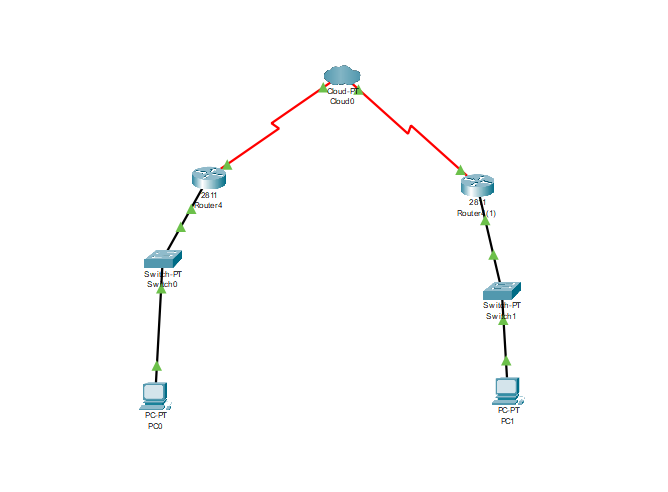
\includegraphics[width=0.8\textwidth]{P1/img/Screenshot 2025-06-12 174011.png}
\end{figure}

\begin{figure}[H]
\centering
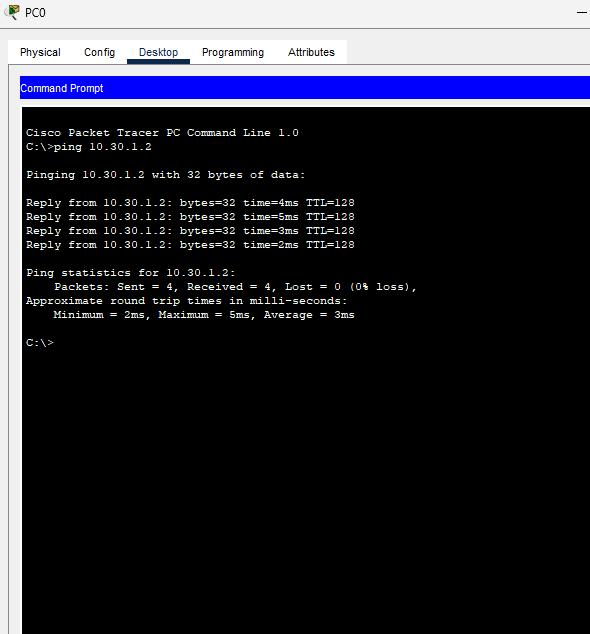
\includegraphics[width=0.8\textwidth]{P1/img/Screenshot 2025-06-12 175509.png}
\end{figure}

\begin{figure}[H]
\centering
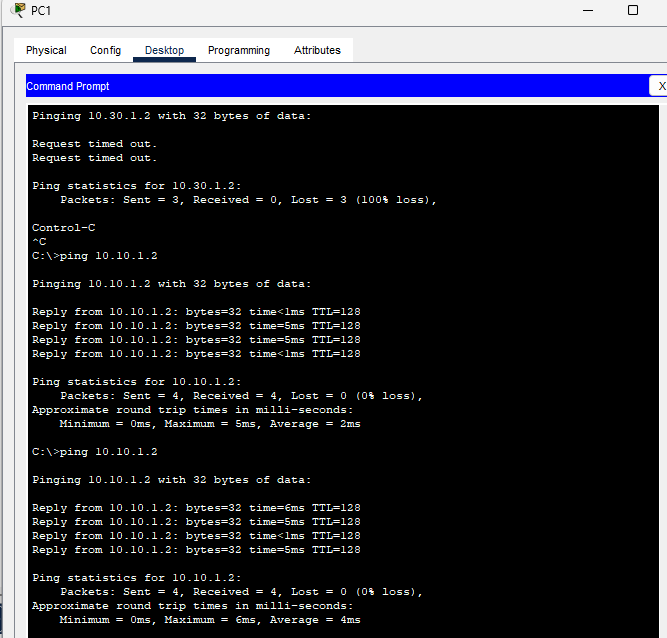
\includegraphics[width=0.8\textwidth]{P1/img/Screenshot 2025-06-12 174545.png}
\end{figure}

Point-to-Point Tunneling Protocol (PPTP) berfungsi sebagai protokol VPN yang memungkinkan klien untuk terhubung secara aman ke jaringan lokal router melalui internet. Dalam jaringan praktikum ini, PPTP digunakan untuk membuat tunnel atau jalur komunikasi virtual antara PC klien dan router, sehingga klien mendapatkan alamat IP lokal dan dapat berkomunikasi dengan perangkat lain di jaringan internal seolah-olah terhubung langsung. Fungsi ini memungkinkan akses jarak jauh yang aman dan pengelompokan jaringan antar perangkat, serta memberikan lapisan keamanan tambahan dengan mengenkripsi data yang dikirim melalui koneksi VPN.


\section{Kesimpulan}
Dari praktikum ini dapat disimpulkan bahwa:

\begin{itemize}
    \item Praktikan berhasil melakukan konfigurasi VPN PPTP pada Router MikroTik yang memungkinkan PC1 terhubung secara aman ke jaringan lokal router.
    \item Konfigurasi DHCP, NAT, dan IP address pada router berjalan dengan baik dan sesuai kebutuhan modul.
    \item QoS melalui fitur Simple Queue berhasil digunakan untuk membatasi bandwidth jaringan lokal.
    \item Percobaan ini memberikan pemahaman praktis mengenai manajemen jaringan menggunakan MikroTik dan pentingnya konfigurasi VPN serta pengaturan bandwidth.
\end{itemize}
\section{Lampiran}
\subsection{Dokumentasi saat praktikum}
\begin{figure}[H]
\centering
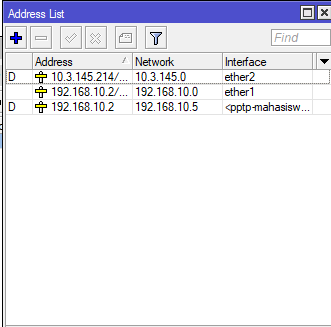
\includegraphics[width=0.8\textwidth]{P1/img/Screenshot 2025-06-05 190731.png}
\end{figure}

\begin{figure}[H]
\centering
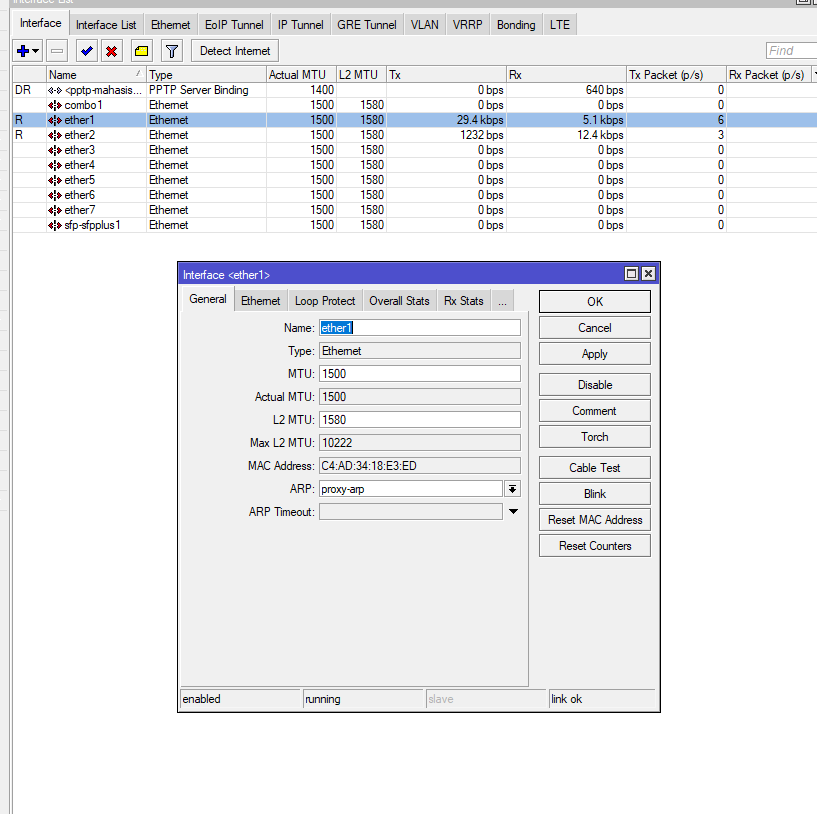
\includegraphics[width=0.8\textwidth]{P1/img/Screenshot 2025-06-05 190802.png}
\end{figure}

\begin{figure}[H]
\centering
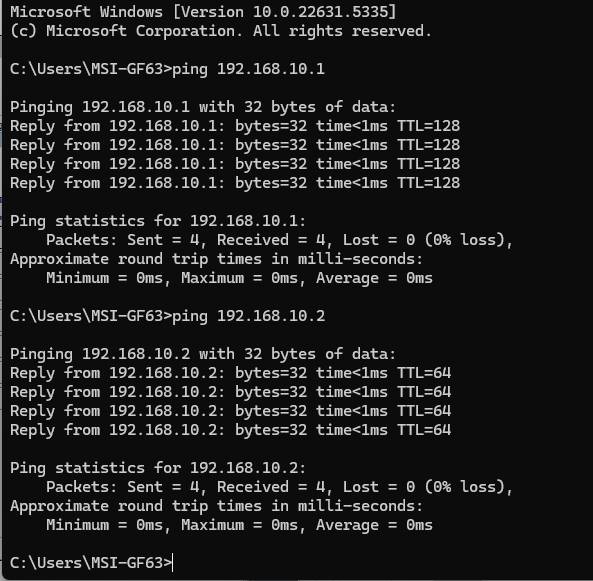
\includegraphics[width=0.8\textwidth]{P1/img/Screenshot 2025-06-05 191047.png}
\end{figure}
\begin{figure}[H]
\centering
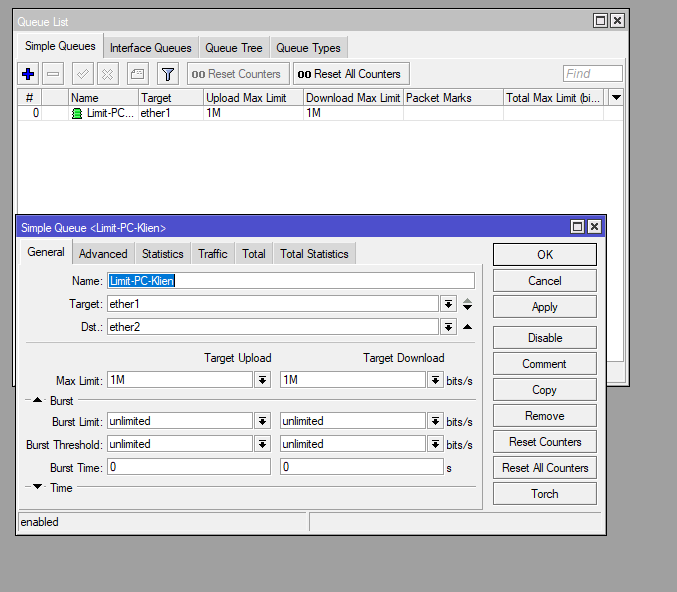
\includegraphics[width=0.8\textwidth]{P1/img/Screenshot 2025-06-05 191336.png}
\end{figure}
\begin{figure}[H]
\centering
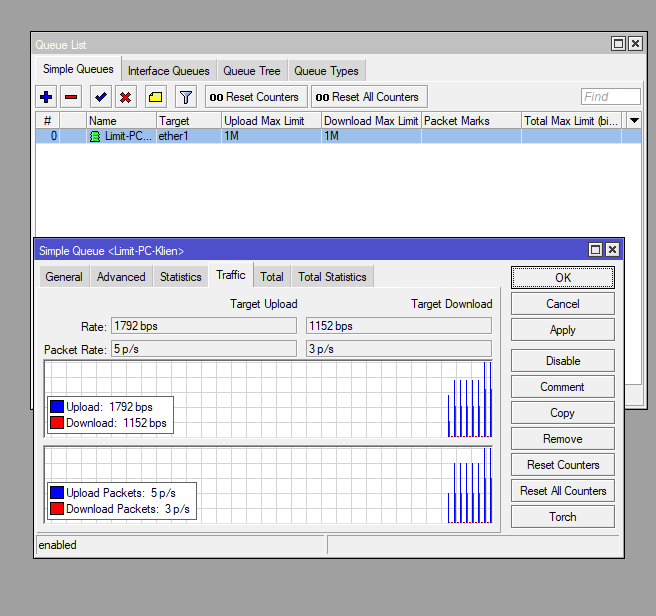
\includegraphics[width=0.8\textwidth]{P1/img/Screenshot 2025-06-05 191431.png}
\end{figure}
\begin{figure}[H]

\centering
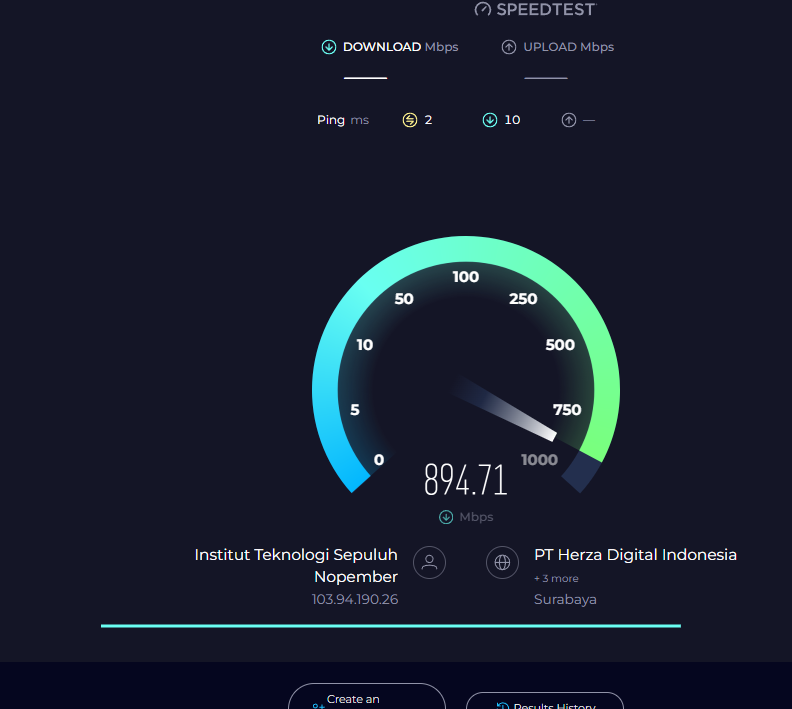
\includegraphics[width=0.8\textwidth]{P1/img/Screenshot 2025-06-05 191601.png}
\end{figure}
\begin{figure}[H]

\centering
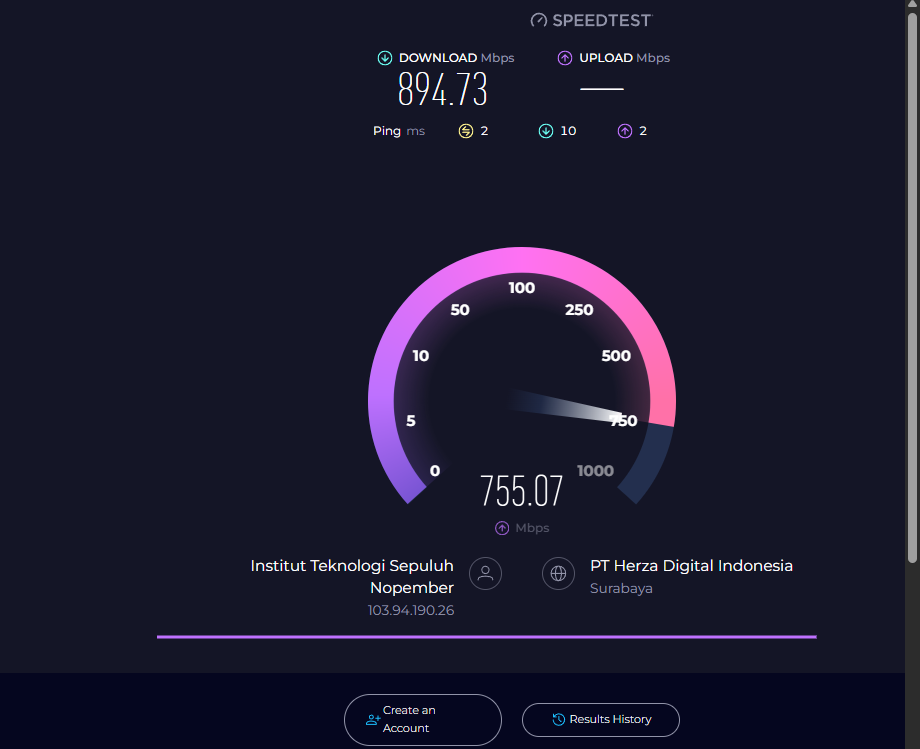
\includegraphics[width=0.8\textwidth]{P1/img/Screenshot 2025-06-05 191620.png}
\end{figure}
\begin{figure}[H]

\centering
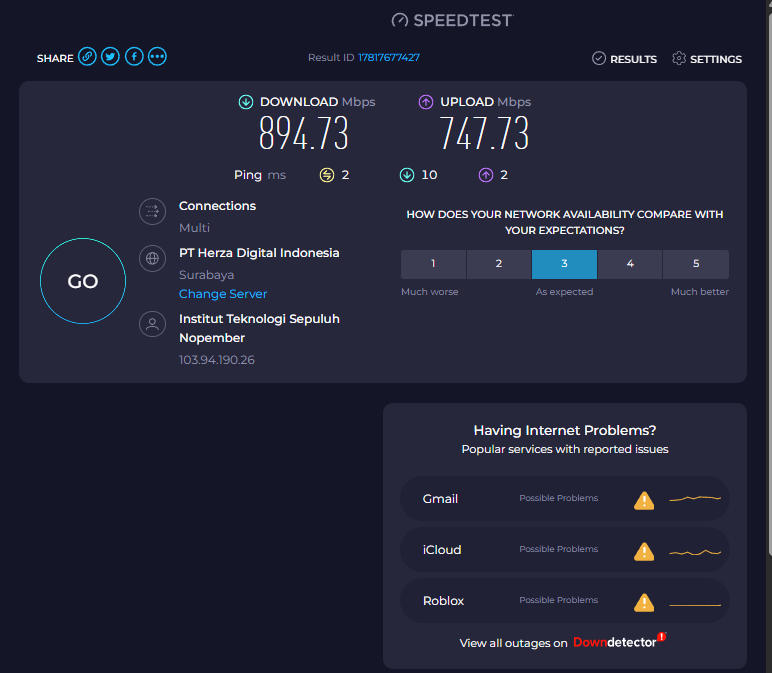
\includegraphics[width=0.8\textwidth]{P1/img/Screenshot 2025-06-05 191624.png}
\end{figure}
\begin{figure}[H]

\centering
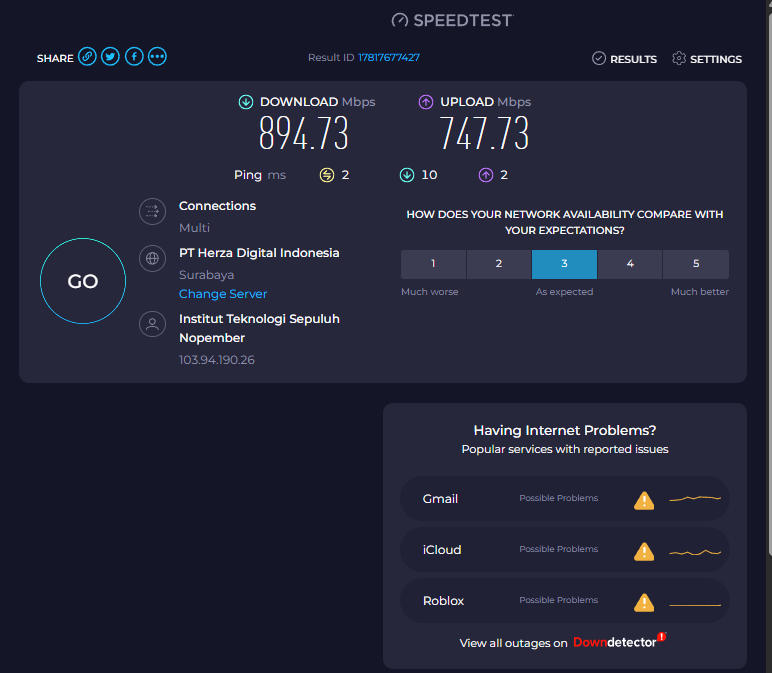
\includegraphics[width=0.8\textwidth]{P1/img/Screenshot 2025-06-05 191624.png}
\end{figure}

\begin{figure}[H]

\centering
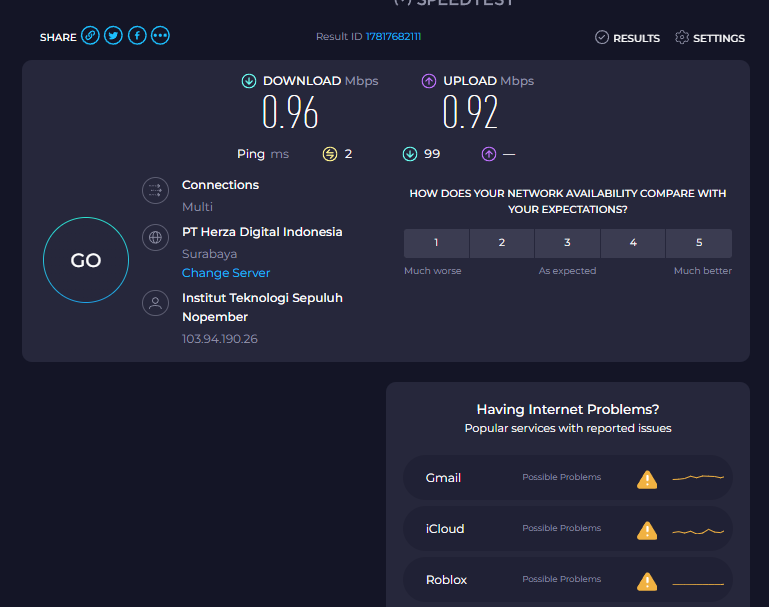
\includegraphics[width=0.8\textwidth]{P1/img/Screenshot 2025-06-05 191803.png}
\end{figure}

\begin{figure}[H]
\centering
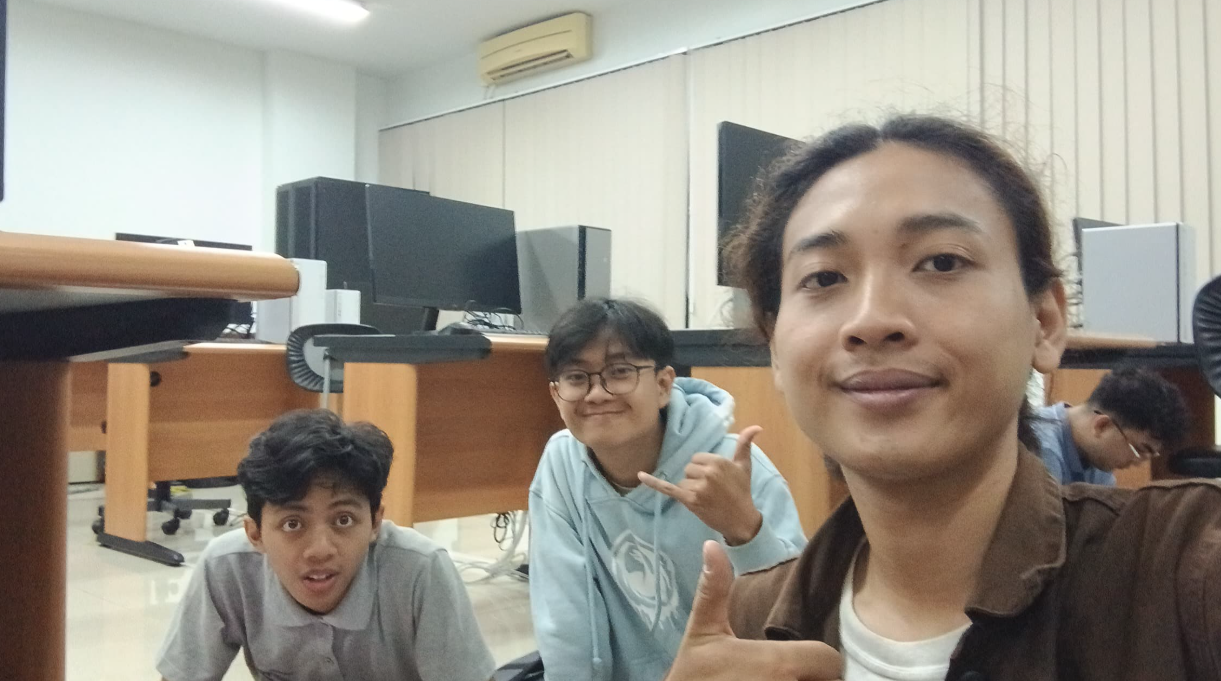
\includegraphics[width=0.8\textwidth]{P1/img/image.png}
\end{figure}



